\subsubsection{27.03.15 (Competition)}
\begin{center}
	1-st day of competition "FTC Dutch Open" in Eindhoven.
\end{center}

Today there was technical day. Also today we presented our engineering book to judges.\newline

As soon as we arrived at competition area, two of us started talking with other FTC teams. There were 48 teams on competition. We learned about opportunities and strategy of every team. We got data about all robots except two robots of teams from Saudi Arabia because their robots didn't arrived at Nederlands yet (they we transported as a luggage on another plane).\newline 
All the teams received from our team lists with short information about our strategy and opportunities. The background of our information list was the same to the background of the print on plexiglass protection of our robot which made our robot more noticable. So we did everything to attract others' teams attention and increase our chanses to be chosen by other teams for final matches.\newline
Between the teams we found two our friends (we kept in touch woth them since the central robofest in Moscow): team "Auto Vortex" from Romania and team "Trex" from Rissia.\newline

At the beginning of the day we presented engineering book. At first one of us told the judges about:
\begin{enumerate}
	\item Our team.
	
	\item Our strategy in game.
	
	\item Construction of the robot.
	
	\item Resourses we used in our work (LaTex, Creo Parametric 3.0, etc).
	
	\item Our coaches and sponsors.
	
\end{enumerate}
After that we all answered the judges' questions. After the presentation we realised, that our new way of telling it is more effective and we decided to follow this way in further presentations.\newline

Improvements that were done:
\begin{enumerate}
	\item It was found that the right corner of the bucket hooks the wire that connect servo that overturns bucket with servocontroller. So the corner was cut and it was glued the patch. The bucket stopped hook the wire.
	\begin{figure}[H]
		\begin{minipage}[h]{0.47\linewidth}
			\center{\includegraphics[scale=0.18]{days/11.02.15/images/01}}
			\caption{The cut corner}
		\end{minipage}
		\hfill
		\begin{minipage}[h]{0.47\linewidth}
			\center{\includegraphics[scale=0.6]{days/11.02.15/images/02}}
			\caption{Larger image}
		\end{minipage}
	\end{figure}
	
	\item We decided to concentrate on the programme of autonomous period from the parking zone because the most part of teams did autonomous period from the ramp better than from the parking zone.
	
		\item The guideway for balls was fixed only on the slats. So it staggered. To prevent this it was decided to install the stopper that that limits backlash of the guiedeway. So the problem was fixed.
	\begin{figure}[H]
		\begin{minipage}[h]{0.2\linewidth}
			\center  
		\end{minipage}
		\begin{minipage}[h]{0.6\linewidth}
			\center{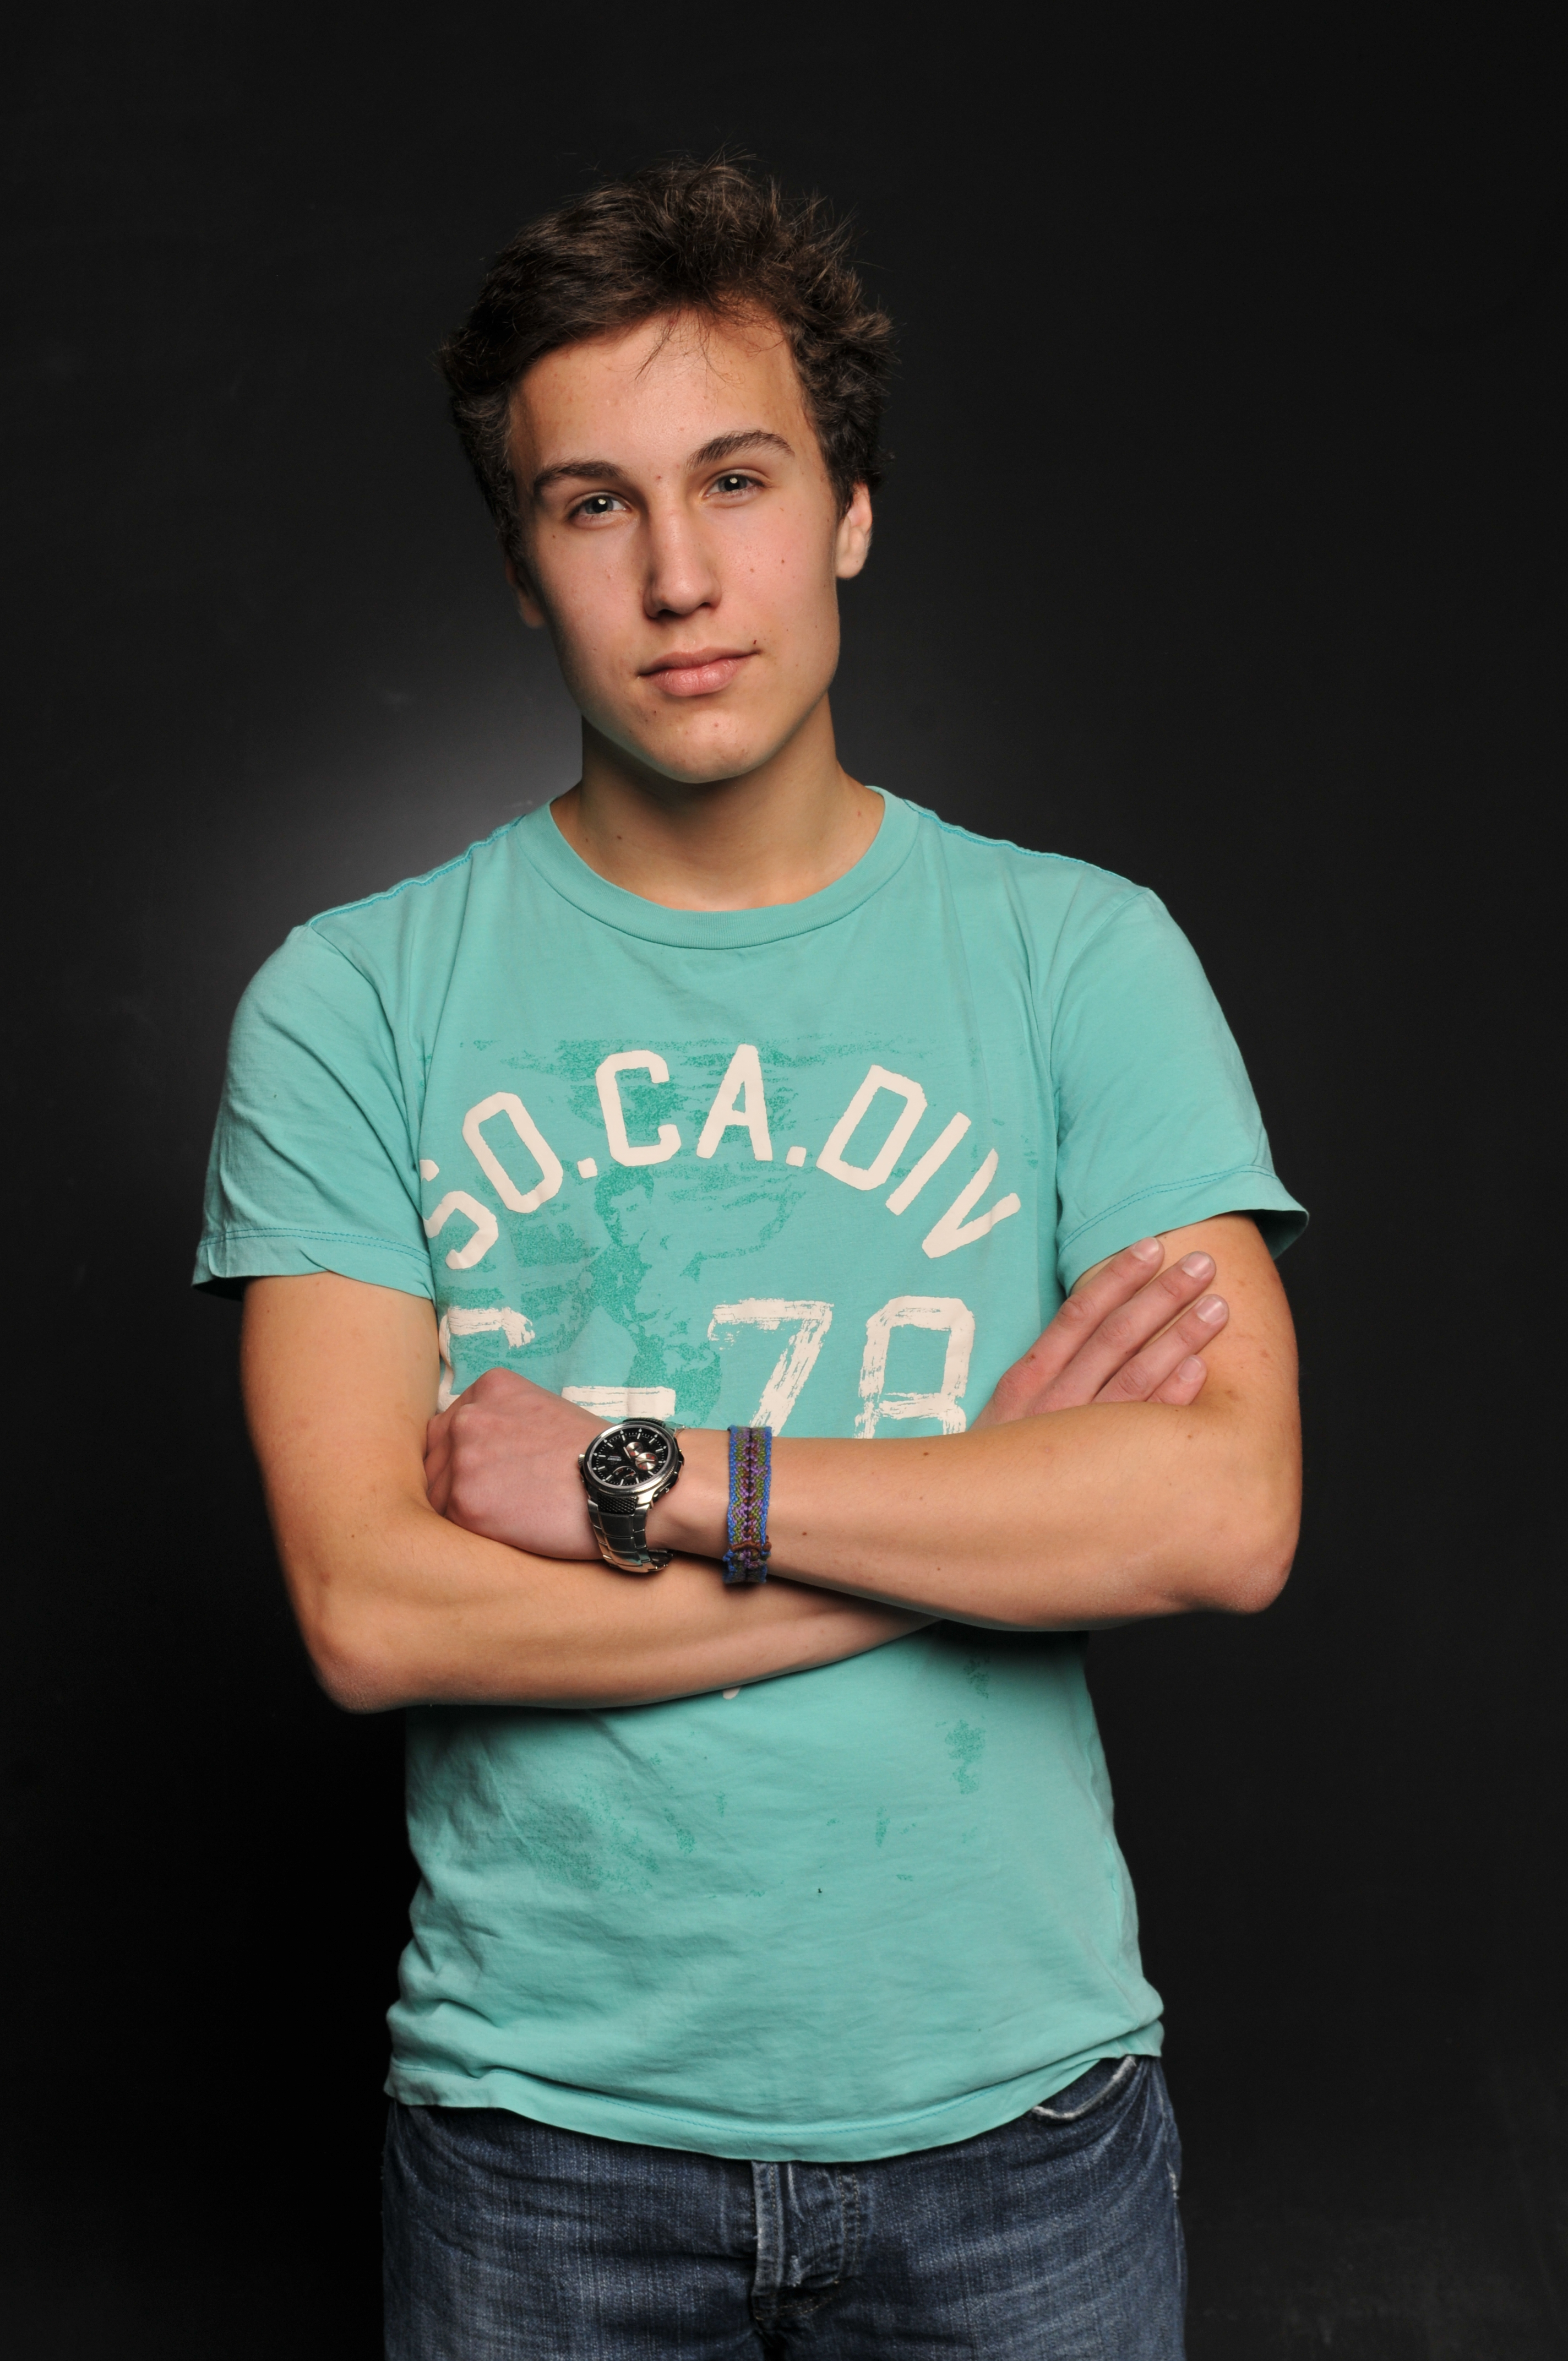
\includegraphics[scale=0.18]{days/11.02.15/images/03}}
			\caption{Stopper}
		\end{minipage}
	\end{figure}
	
\end{enumerate}
\fillpage
